\begin{figure}[t]
\centering
\bgroup
\def\arraystretch{1.8}
\begin{tabular}{c c c c c c c c c c c c}

\multicolumn{4}{c}{
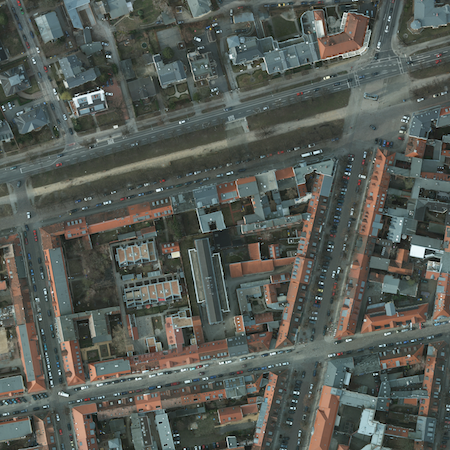
\includegraphics[height=0.277\textwidth]{experiments2_files/545_17_img.png}} & 
\multicolumn{4}{c}{
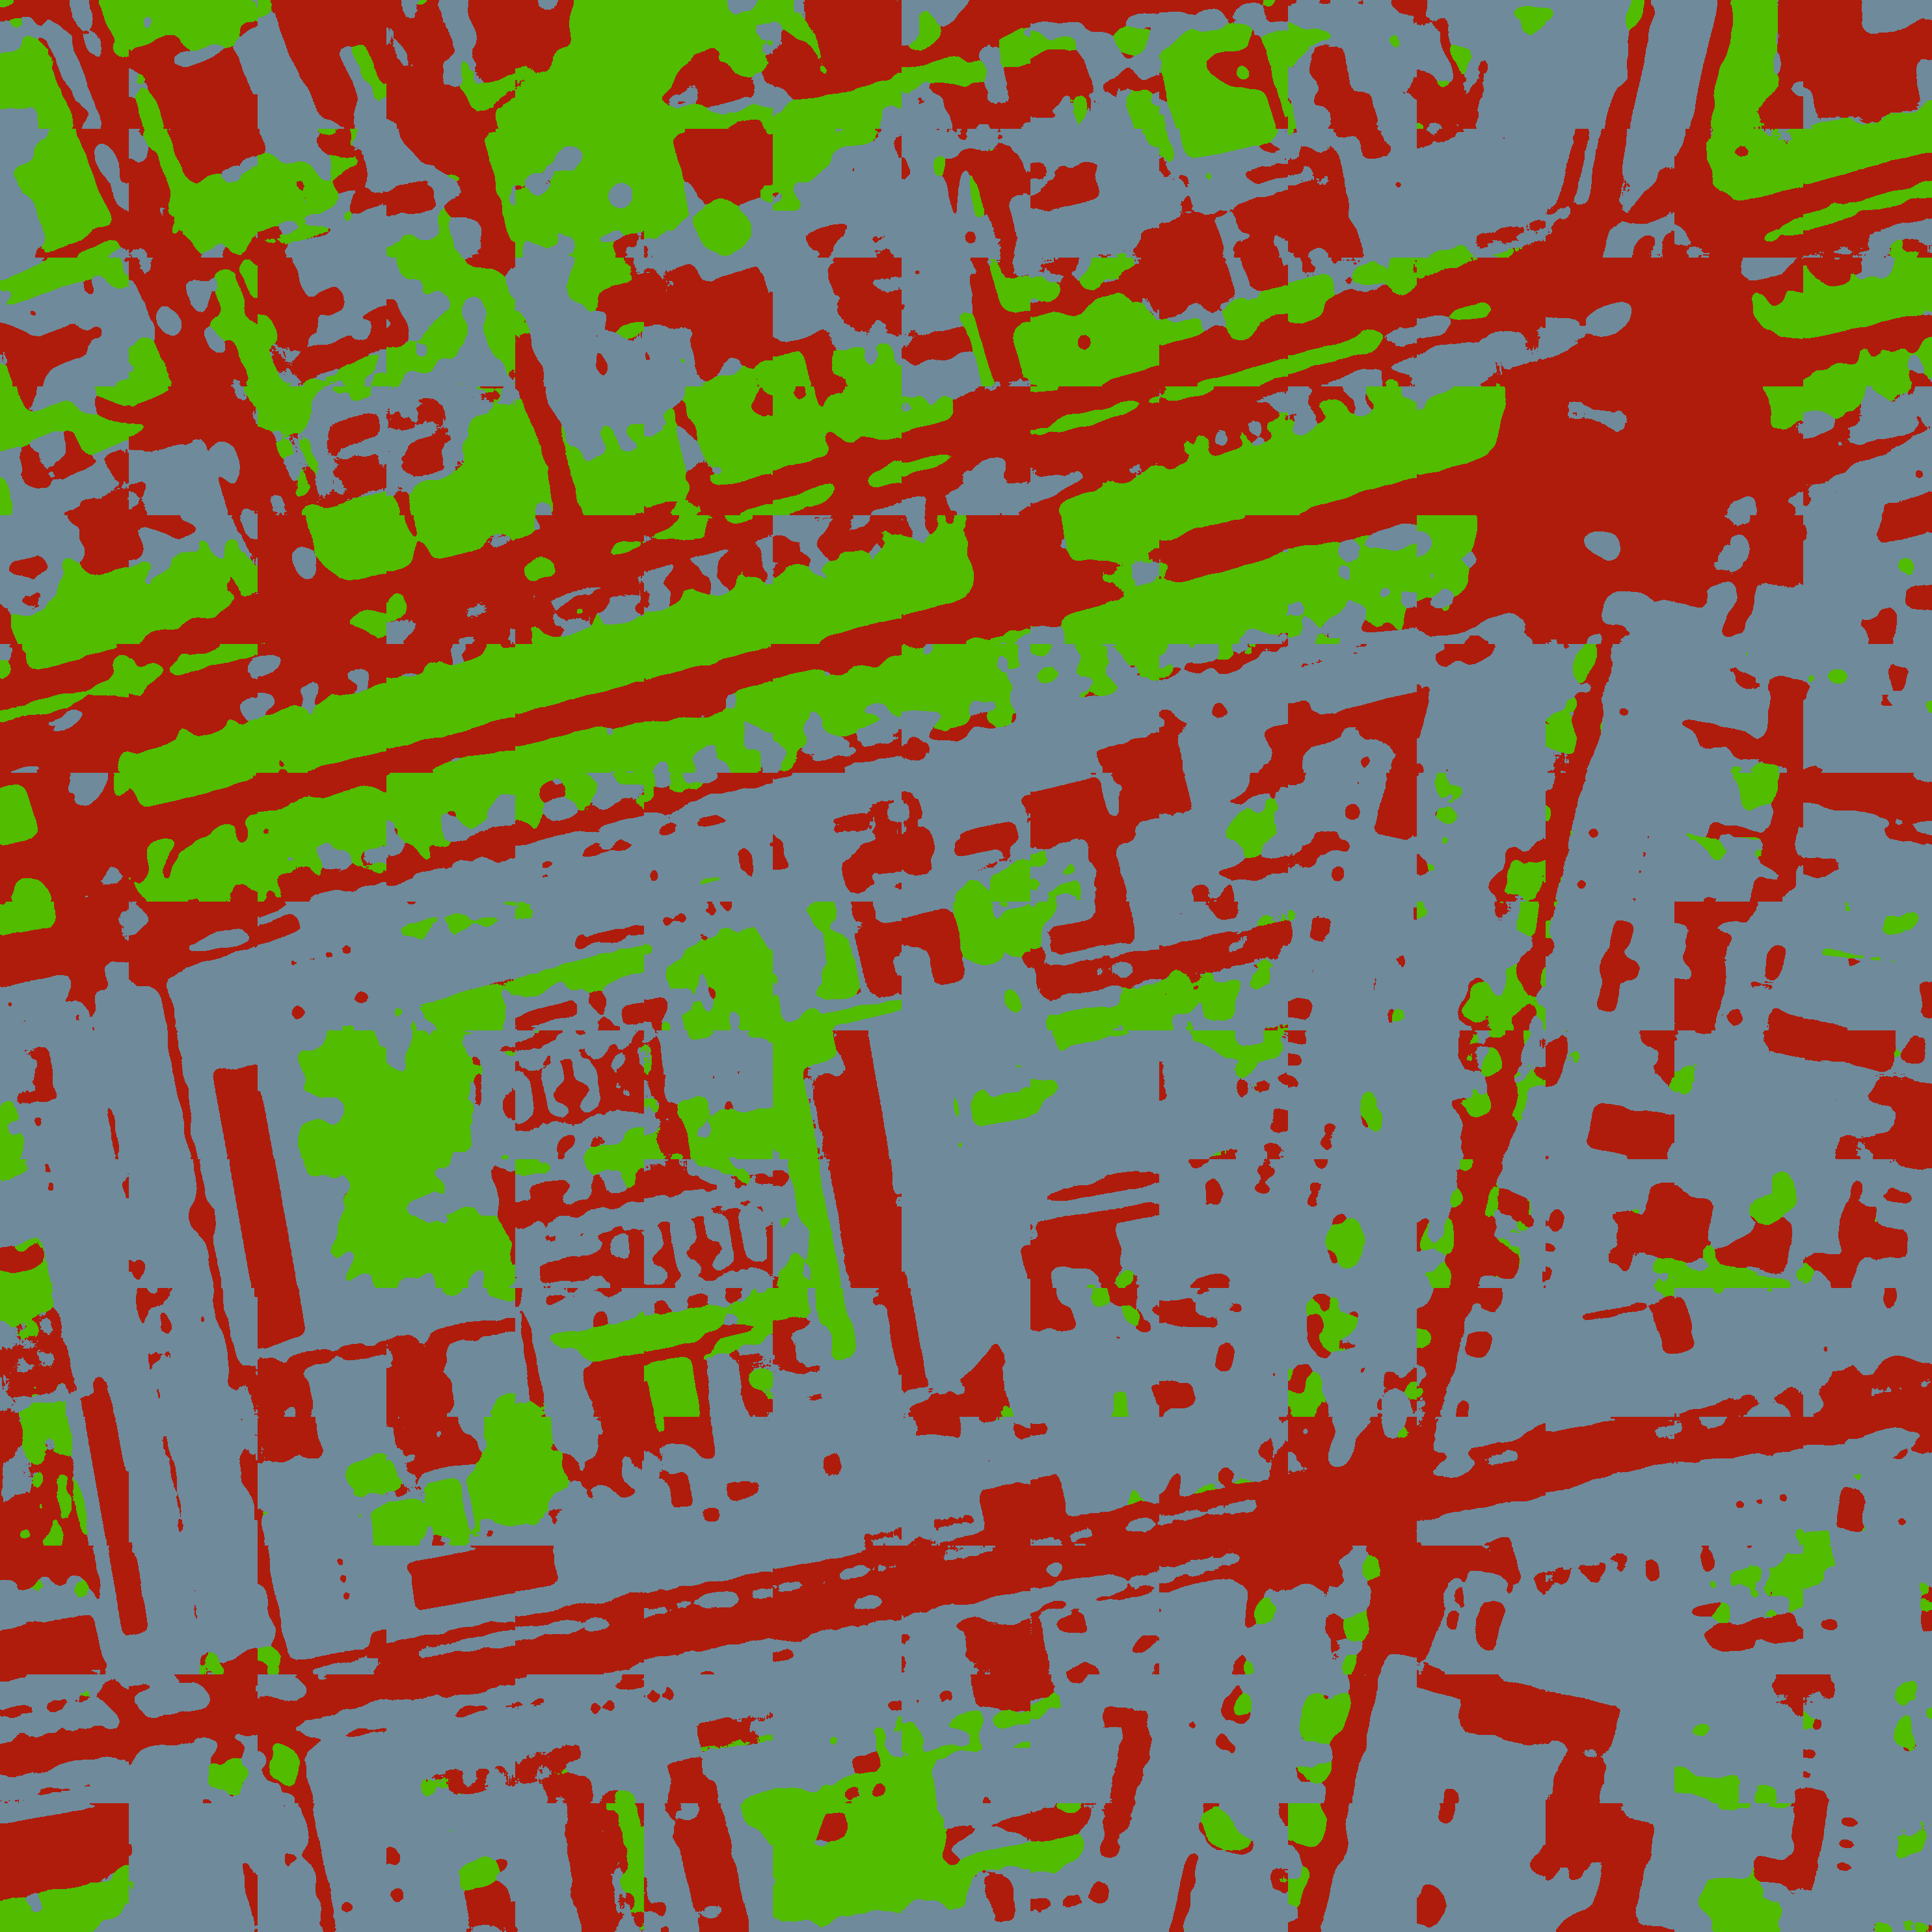
\includegraphics[height=0.277\textwidth]{experiments2_files/545_17_preds.png}} & 
\multicolumn{4}{c}{
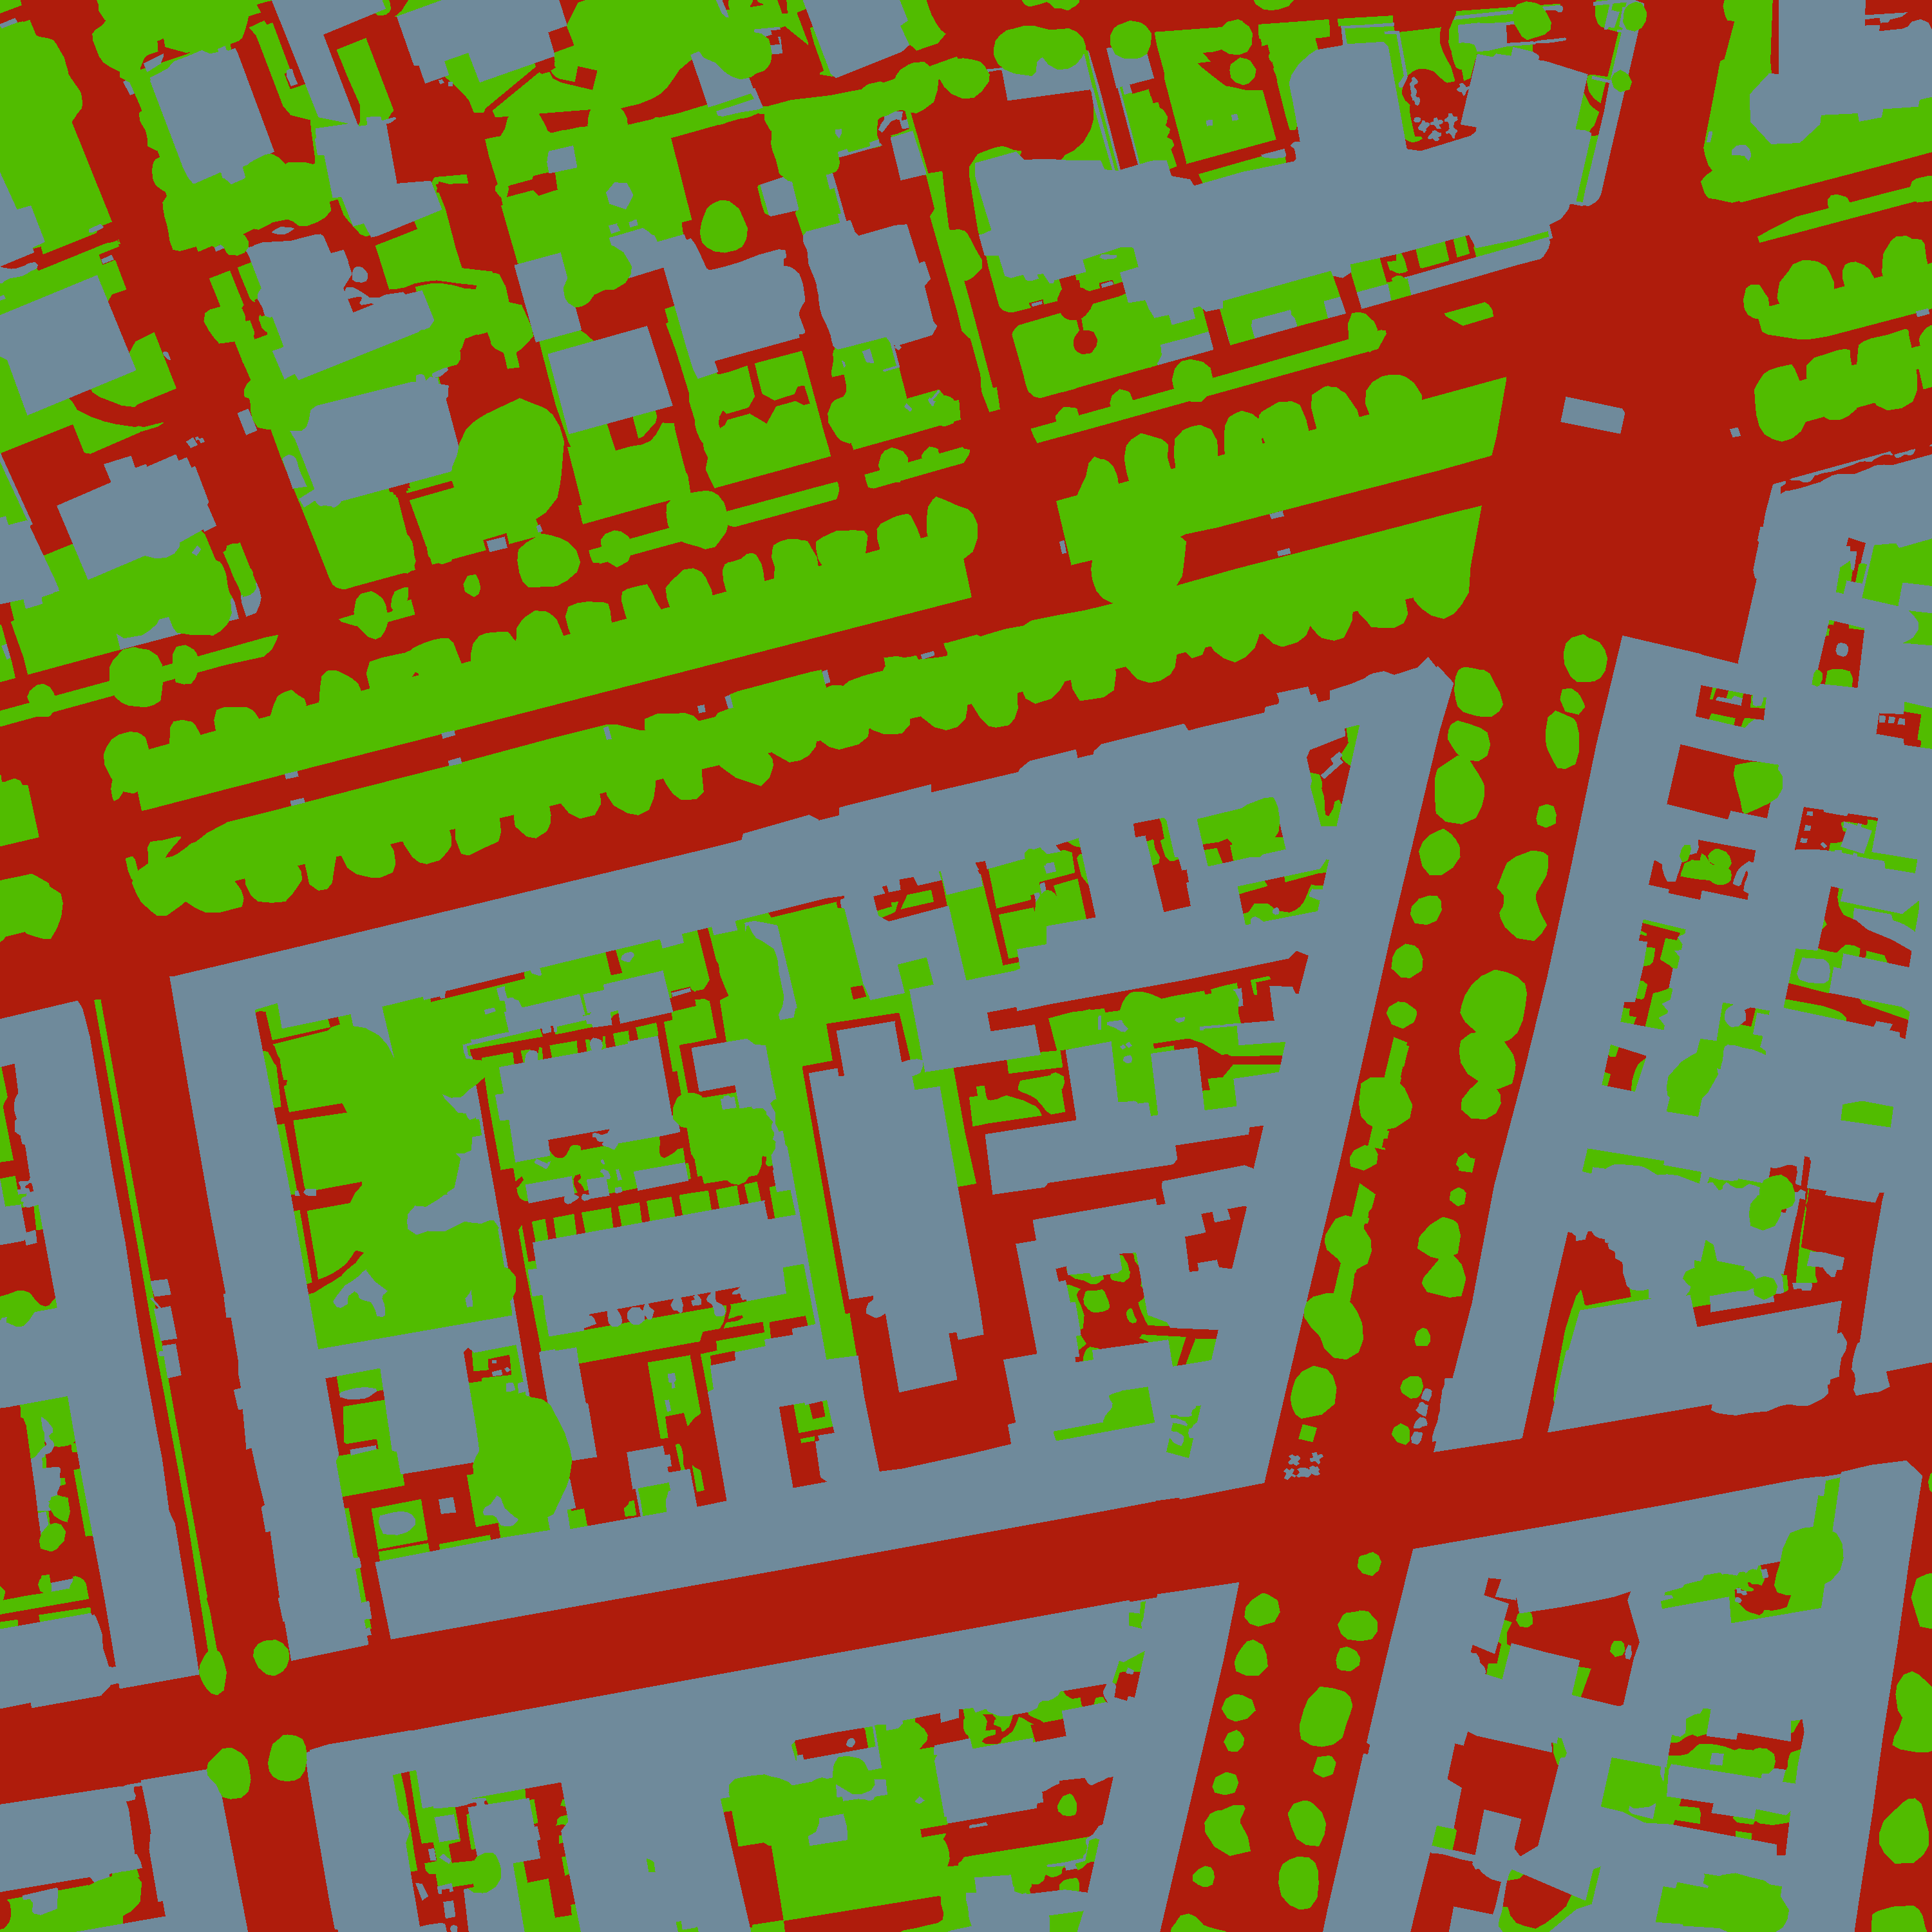
\includegraphics[height=0.277\textwidth]{experiments2_files/545_17_gt.png}} \\

\multicolumn{4}{c}{
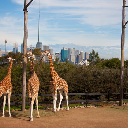
\includegraphics[height=0.277\textwidth]{experiments2_files/509_img_254.png}} & 
\multicolumn{4}{c}{

\includegraphics[height=0.277\textwidth]{experiments2_files/509_reordered_preds_254.png}} & 
\multicolumn{4}{c}{

\includegraphics[height=0.277\textwidth]{experiments2_files/509_targets_254.png}} \\

\multicolumn{3}{c}{
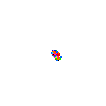
\includegraphics[height=0.20\textwidth]{experiments2_files/556_pointcloud_random.png}} & 
\multicolumn{3}{c}{
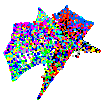
\includegraphics[height=0.20\textwidth]{experiments2_files/556_pointcloud_e_3.png}} & 
\multicolumn{3}{c}{
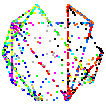
\includegraphics[height=0.20\textwidth]{experiments2_files/556_pointcloud_e_24.png}} &
\multicolumn{3}{c}{
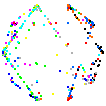
\includegraphics[height=0.20\textwidth]{experiments2_files/247_pointcloud_best.png}}\\

\end{tabular}
\egroup
\caption{\label{f:splash} Fully unsupervised image clustering and segmentation (IID). Top: input, prediction and ground truth for Potsdam-3 and COCO-Stuff-3. Bottom: raw STL10 predictions before, during and after training.}
\end{figure}